\documentclass[a4paper, 11pt]{article}
\usepackage[utf8]{inputenc}
\usepackage{float}
\usepackage{graphicx}
\usepackage{url}
\usepackage{enumitem}
\usepackage{subcaption}

\setlist[itemize]{itemsep=0.5pt, parsep=0.5pt, topsep=0pt, partopsep=0pt}
\setlist[enumerate]{itemsep=0.5pt, parsep=0.5pt, topsep=0pt, partopsep=0pt}

%opening
\title{HW3 Report, Loggy: A Logical Time Logger}
\author{David Fischer}
\date{\today{}}

\begin{document}

\maketitle

\section{Introduction}
% waffle about lamport clocks & vector clocks, their importance in different applications like storage replication

% a bit about what was implemented (central logger with a holdback queue, two clock modules, lamport and vector, workers who send messages between eachother on a random delay with random jitter between sending/recieving and reporting to the logger)

\section{Main problems and solutions}

\subsection{}

% something about difficulties validating if the clocks, especially the vector clocks, are functioning correctly, solved in chart maker with evaluation

\subsection{}

% difficulty reading the log until the log output was made clean using the built in padding

\subsection{}

% holdback queue implementation, difficulty mentally parsing the queue size/why it jumps so massively


\section{Evaluation}

\subsection{Visualization}

To aid evaluation, a module \textit{mermaid} was implemented to create visual representations of the messages flowing between the vector clocks.

See appendix. (TODO, proper sendoff)

\subsection{Delay caused by Jitter Comparison of Lamport and Vector}

% TODO: write some code here to auto-test the lamport & vector clocks to correlate jitter with maximum queue size, should be easy enough
% TODO: actually validate that the queue size isn't too big, logging seems weird right now

% graph here of the two clocks (jitter/queue size)

\section{Conclusions}

% something about vector clocks

\section{Appendix}

Both of these tests were completed using test:run(<module>, 1500, 500).

\subsection{Lamport Clock}
\begin{verbatim}
119> test:run(time, 1500, 500).
loggy: starting with module time
log: s:5   ringo  sending  ( 24) c:1
log: s:5   john   sending  (  6) c:1
log: s:5   george sending  ( 26) c:1
log: s:2   paul   received ( 24) c:2
log: s:2   john   received ( 26) c:2
log: s:2   paul   received (  6) c:3
log: s:2   john   sending  ( 50) c:3
log: s:2   ringo  received ( 50) c:4
log: s:2   john   sending  ( 73) c:4
log: s:2   paul   sending  ( 28) c:4
log: s:8   george received ( 28) c:5
log: s:8   ringo  sending  (  2) c:5
log: s:8   john   sending  ( 37) c:5
log: s:13  george received ( 73) c:6
log: s:13  paul   received (  2) c:6
log: s:13  john   sending  (  1) c:6
log: s:3   george sending  ( 48) c:7
log: s:3   paul   sending  ( 30) c:7
log: s:3   ringo  received ( 48) c:8
log: s:3   paul   received ( 37) c:8
log: s:3   ringo  sending  ( 86) c:9
log: s:3   george received ( 86) c:10
log: s:3   george received ( 30) c:11
log: s:3   george sending  ( 85) c:12
log: s:3   ringo  received ( 85) c:13
log: s:3   ringo  sending  ( 83) c:14
log: s:3   george received ( 83) c:15
log: s:3   ringo  received (  1) c:15
\end{verbatim}

\begin{figure}[H]
  \begin{center}
    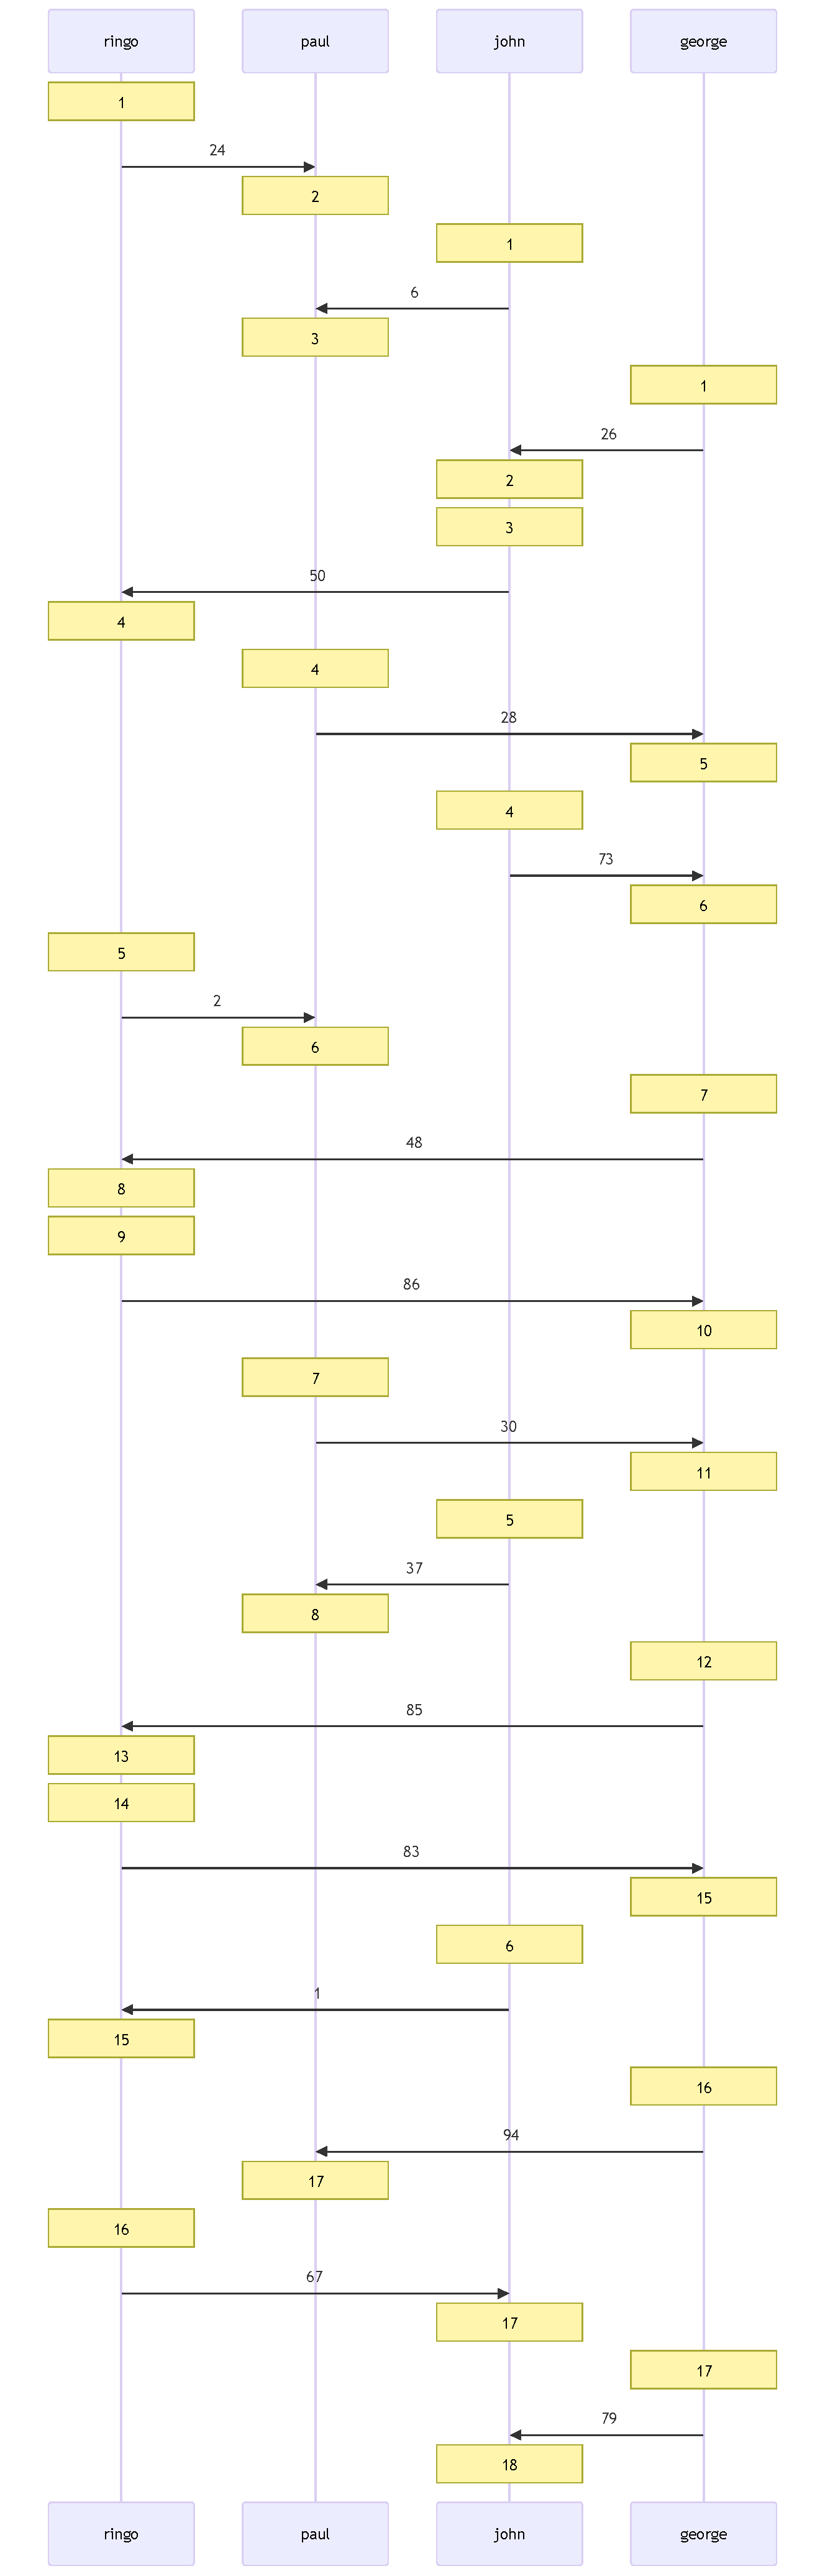
\includegraphics[height=\textheight]{graphics/mermaid_lamport.pdf}
    \caption{Sequence visualization of the Lamport timestamp algorithm}
    \label{fig:seq1}
  \end{center}
\end{figure}

\subsection{Vector Clock}
\begin{verbatim}
120> test:run(vect, 1500, 500).
loggy: starting with module vect
log: s:1   ringo  sending  ( 24) c:ringo => 1
log: s:1   paul   received ( 24) c:paul => 1,ringo => 1
log: s:0   john   sending  (  6) c:john => 1
log: s:0   paul   received (  6) c:john => 1,paul => 2,ringo => 1
log: s:0   george sending  ( 26) c:george => 1
log: s:0   john   received ( 26) c:john => 2,george => 1
log: s:0   john   sending  ( 50) c:john => 3,george => 1
log: s:0   ringo  received ( 50) c:john => 3,ringo => 2,george => 1
log: s:2   john   sending  ( 73) c:john => 4,george => 1
log: s:0   paul   sending  ( 28) c:john => 1,paul => 3,ringo => 1
log: s:0   george received ( 28) c:john => 1,paul => 3,ringo => 1,george => 2
log: s:0   george received ( 73) c:john => 4,paul => 3,ringo => 1,george => 3
log: s:0   ringo  sending  (  2) c:john => 3,ringo => 3,george => 1
log: s:0   paul   received (  2) c:john => 3,paul => 4,ringo => 3,george => 1
log: s:0   george sending  ( 48) c:john => 4,paul => 3,ringo => 1,george => 4
log: s:0   ringo  received ( 48) c:john => 4,paul => 3,ringo => 4,george => 4
log: s:1   john   sending  ( 37) c:john => 5,george => 1
log: s:1   paul   received ( 37) c:john => 5,paul => 5,ringo => 3,george => 1
log: s:0   ringo  sending  ( 86) c:john => 4,paul => 3,ringo => 5,george => 4
log: s:0   george received ( 86) c:john => 4,paul => 3,ringo => 5,george => 5
log: s:2   george sending  (  8) c:john => 4,paul => 3,ringo => 5,george => 6
log: s:1   ringo  sending  ( 84) c:john => 4,paul => 3,ringo => 6,george => 4
log: s:1   paul   received ( 84) c:john => 5,paul => 6,ringo => 6,george => 4
log: s:1   paul   received (  8) c:john => 5,paul => 7,ringo => 6,george => 6
log: s:1   paul   sending  ( 46) c:john => 5,paul => 8,ringo => 6,george => 6
log: s:1   george received ( 46) c:john => 5,paul => 8,ringo => 6,george => 7
log: s:1   john   sending  (  1) c:john => 6,george => 1
log: s:1   ringo  received (  1) c:john => 6,paul => 3,ringo => 7,george => 4
log: s:0   george sending  ( 99) c:john => 5,paul => 8,ringo => 6,george => 8
log: s:0   paul   received ( 99) c:john => 5,paul => 9,ringo => 6,george => 8
\end{verbatim}

\begin{figure}[H]
  \begin{center}
    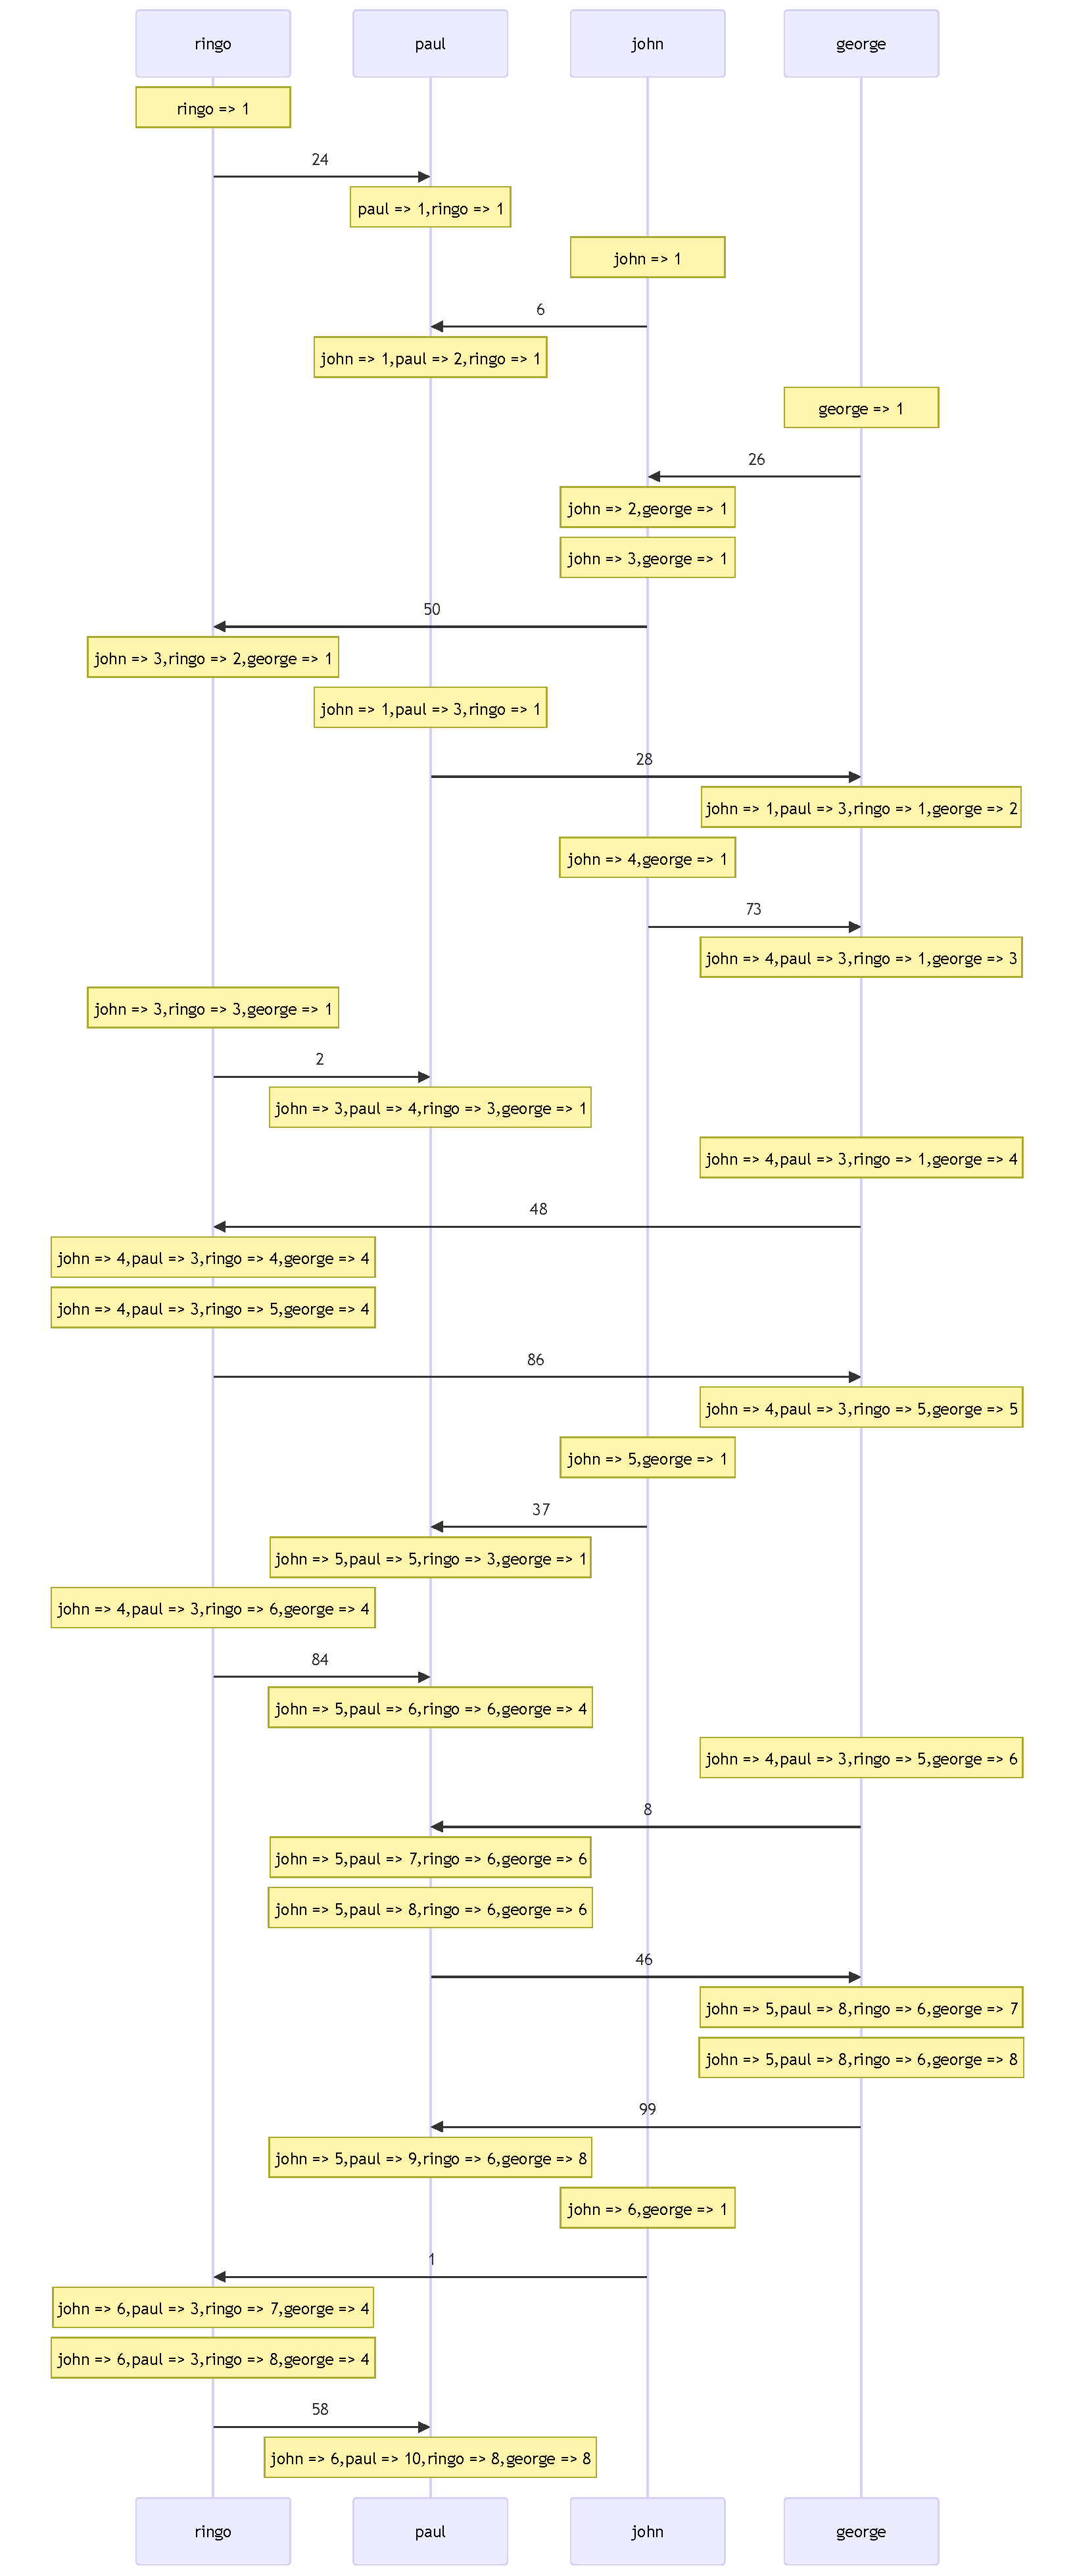
\includegraphics[height=\textheight]{graphics/mermaid_vector.pdf}
    \caption{Sequence visualization of the vector clock implementation}
    \label{fig:seq2}
  \end{center}
\end{figure}

\end{document}
